O metodo de floresta aleatória também é amplamente utilizado para modelos de classificação , mas antes entender este tipo de modelo precisamos passar primeiro por outros conceitos importantes.


\subsubsection{Árvores de decisão}

Uma árvore de decisão é um método supervisionado e não paramétrico.

Estes métodos tem uma representação gráfica baseada em árvores, e a ideia é agrupar indíviduos em grupos com características similares. Ese agrupamento é feito a partir de diversas repartições do banco de dados com base nas características das variáveis.


Uma das formas mais simples de entender o processo de uma árvore de decisão é através de sua representação gráfica:


\begin{figure}
\centering
\caption{Exemplicifação de uma árvore de decisão}
  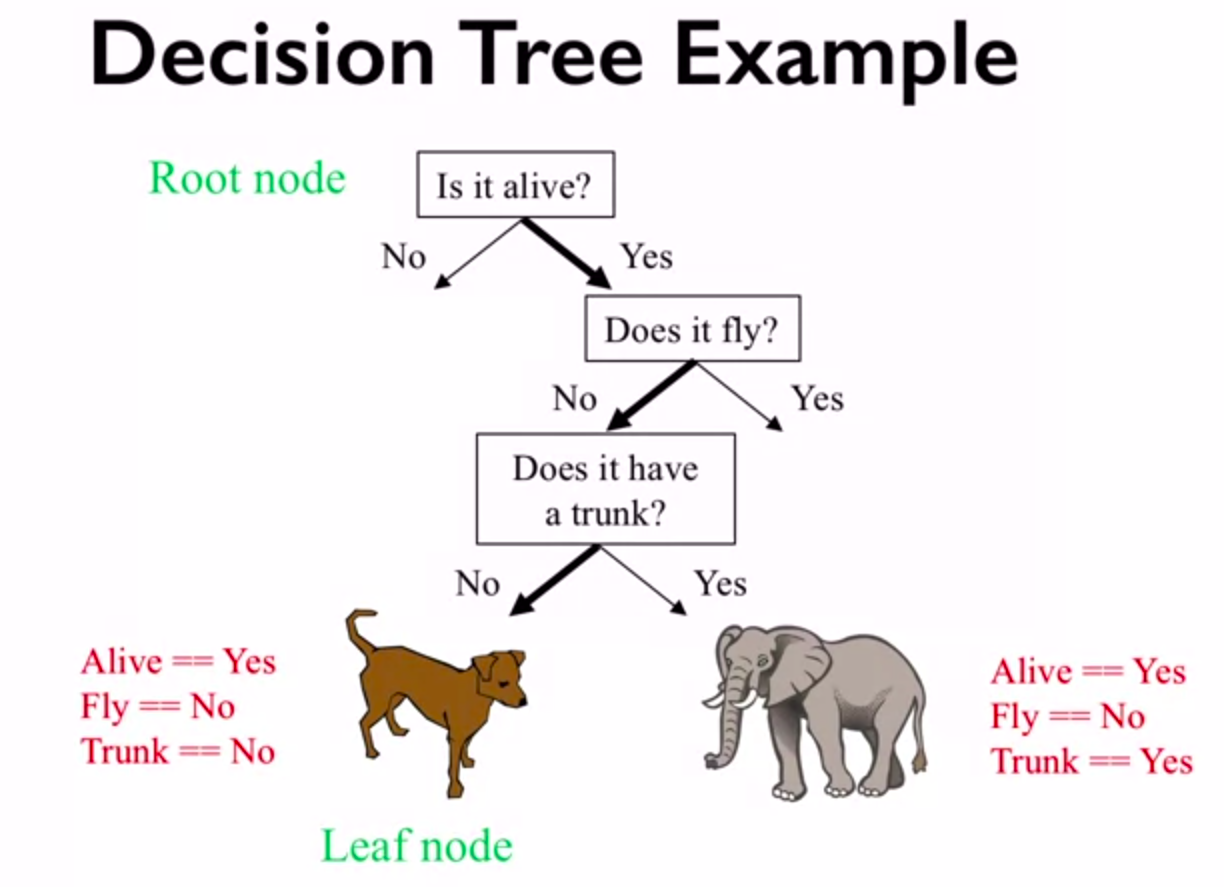
\includegraphics[width=8cm]{"images/dTreeExample.png"}
  %\centering
\caption*{Fonte: }%%"https://machine-learning-and-data-science-with-python.readthedocs.io/en/latest/assignment5_sup_ml.html"}
  \label{dTree}
\end{figure} 

O exemplo em %\ref{dTree} fshgf




\begin{itemize}

\item As divisões da amostra resultam em subamostras, conhecidas como nós de decisão, ou nó intermediário, ou nó pai, que quando dividido criará novos nós conhecidos como filhos.
\item Quando alguma amostra não puder mais ser dividida por algum critério de parada, ela será conhecida como nó final ou nó folha.

\end{itemize}


\subsubsection{ensemble}


\subsubsection{Floresta Aleatória}



Dizendo de modo simples: o algoritmo de florestas aleatórias cria várias árvores de decisão e as combina para obter uma predição com maior acurácia e mais estável.
